\section{Basics of feedback control}
In general a system is controlled by feedback when its next input value is (partially) determined by its previous output(s). The reason for taking the previous output into account while coming up with a next input is due to external forces that may impacting the system in unexpected ways. These external forces do not come regularly, are not predictable and are also not equally strong each time, hence a notion of uncertainty in the system's behavior occurs. Due to this uncertainty, a model that accurately calculates the system's next input either does not exist or would be too complex. The solution for incorporating the uncertainty from external forces is to use a feedback cycle around the system: the system's output (affected by both the system's input and any external forces) is measured and compared to a desired reference value, after which their difference is transformed into the system's next input.

Important to mention here early on is that controlling a system with a feedback cycle is not a solution to optimization problems. Tasks like ``\textit{Make the flow through the system as large as possible}'' cannot be accomplished with feedback loops \cite{janert2013-feedback}, as they compare the system's current output with a known reference value. Tasks like this require some kind of optimization strategy that determines the reference value, after which a feedback loop can be used to bring and keep the system's output in this desired state.

The input and output of a feedback controlled system are not to be confused with the actual input and output of this system. The air conditioning or heating system has an actual output of hot or cool air, whereas the feedback system's output can be any other measurable metric such as the new temperature after the actual output is applied or the temperature difference caused by the actual output. The input and output of a feedback controlled system are often referred to \textit{control input} and \textit{control output}.

\subsection{Calculating the next control input}
Every time the control output produces a new value, it is compared to a reference value or \textit{setpoint} for it to calculate the \textit{tracking error} as the deviation of the control output from the setpoint:

\begin{equation} \label{eq:tracking-error}
\text{tracking error} = \text{setpoint} - \text{control output}
\end{equation}

This tracking error is then transformed into the next control input by the \textit{controller}. When the tracking error is positive (thus the control output is less than the setpoint), the controller has to produce a new control input that ultimately raises the control output to the same level as the setpoint, such that the tracking error becomes zero. Of course this depends on the \textit{directionality} of the system: for some systems the control input needs to be lowered for the system output to be raised. The controller must be able to make this distinction and therefore has to know the directionality of the system. For example, a heating system requires the controller to \emph{raise} the control input to get a higher temperature, whereas a cooling system requires the controller to \emph{lower} the control input to get a higher temperature.

Besides the directionality, the controller also needs to decide on the magnitude of the correction. If the magnitude is too high, the controller could overcompensate and turn a positive tracking error into a negative tracking error and vice versa, causing the system to oscillate between two states. The worst situation occurs when the negative tracking error caused by the overcompensation of the positive tracking error is larger than the positive tracking error: this results in an ever growing amplitude of the oscillation, which eventually makes the whole system unstable and in the end causes it to blow up.

On the other hand, the magnitude can be too low, causing the controller to undercompensate. This causes tracking errors to persist for a longer time than necessary and makes the system respond slow to disturbances. Although this is less dangerous than instability, this slow behavior is unsatisfactory as well.

In general we require the controller to take in a tracking error and come up with a new control input such that the tracking error will go to zero as soon as possible. For this it turns out that the controller does not need to know anything about the controlled system, but only requires information about the directionality of the system and the magnitude of the correction.

\subsection{Architectural overview}
The architecture of a feedback system is usually depicted as a set of boxes connected with arrows. This way we get a quick overview of the design without worrying about the exact implementation of the various components. The general architecture of a feedback system as discussed above is shown in \Cref{fig:feedbackArchitecture}. Notice that here the control output is negated on the way back and is then added to the setpoint in order to calculate the tracking error. This is common practice as some more preprocessing is required before comparing the control output with the setpoint. For example, the output may contain noise which needs to be smoothened by some kind of filter. Of course preprocessing steps will also be drawn in this overview if applicable.

\begin{figure}[H]
	\begin{center}
		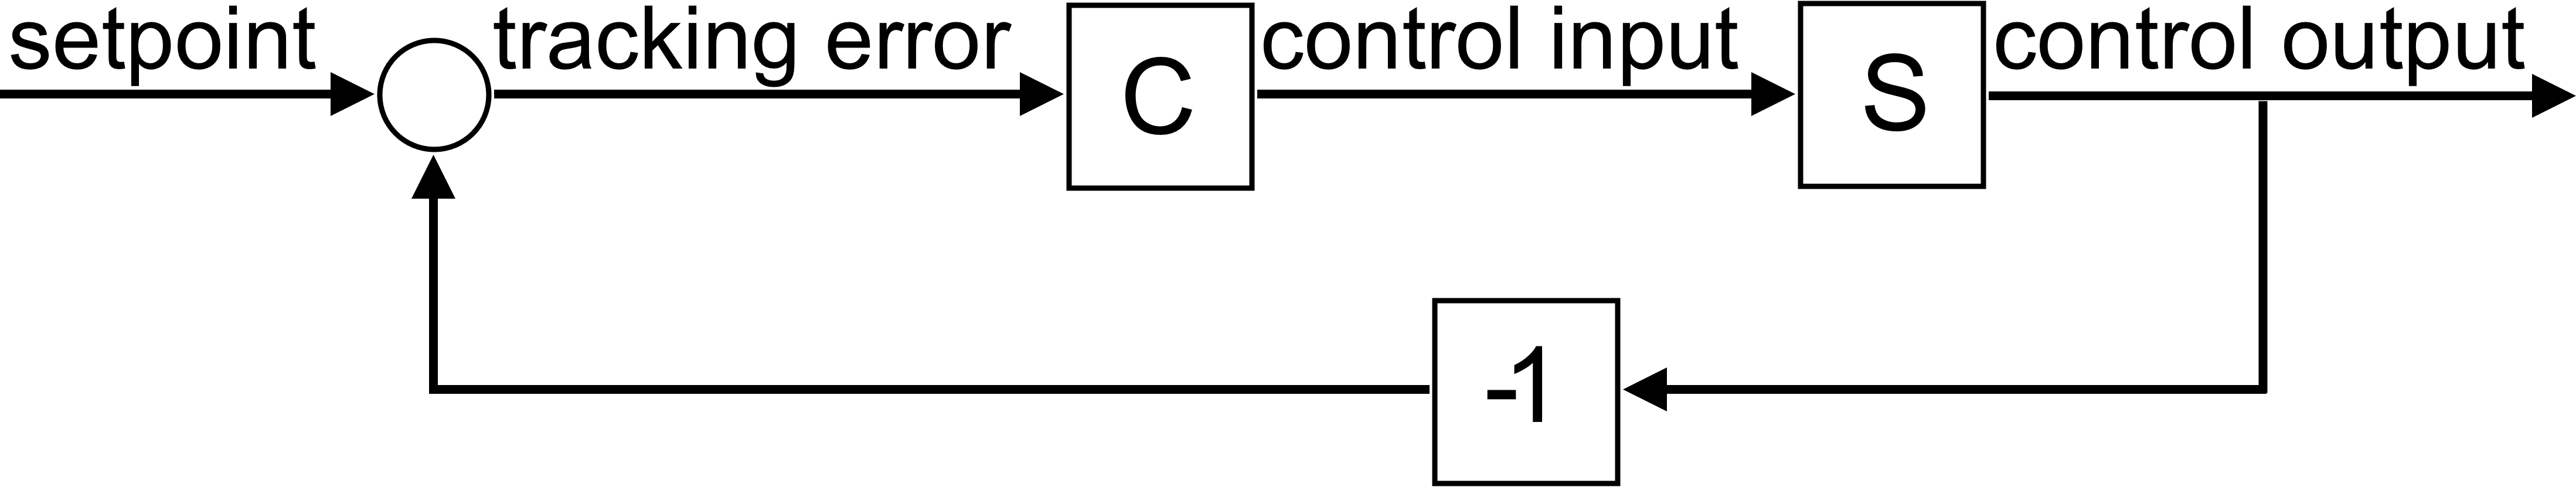
\includegraphics[width=0.85\textwidth]{figures/FeedbackBig.png}
	\end{center}
	\caption{The architecture of a feedback control system}
	\label{fig:feedbackArchitecture}
\end{figure}

Besides these filters, a controller may consist of multiple components by itself. When using an incremental controller, only the difference in the control input is outputted. For the actual input we need to maintain a running sum of all the previous controller outputs and in that way calculate the actual control inputs. Usually these extra steps are also depicted in the architectural overview as extra boxes and arrows.
